\documentclass[onlymath]{beamer}

\usefonttheme{serif}

\usepackage{graphics}
\usepackage{color}
%\usepackage{units}
\usepackage{amsmath}
\usepackage{pgfplots}
\usepackage{tcolorbox}
\usepackage{fancybox}

\usepackage{tikz}
\usetikzlibrary{shapes.geometric}

\usecolortheme{orchid}
\usetheme{boxes}
\setbeamertemplate{navigation symbols}{}%remove navigation symbols
\useoutertheme{infolines}
\useinnertheme{circles}

\setbeamercolor{itemize item}{fg=black}
\setbeamercolor{item}{fg=black}
%\setbeamercovered{invisible}

\providecommand{\e}[1]{\ensuremath{\times 10^{#1}}}

\title[Recent Advancements in AKMC]
  {Recent Advancements in Adaptive Kinetic Monte Carlo}
\author[Sam Chill]{Samuel T. Chill and Graeme Henkelman}

\institute[University of Texas]{Henkelman Group\\
           Department of Chemistry\\
           The University of Texas at Austin}

\begin{document}

\begin{frame}
  \titlepage{}
\end{frame}

\begin{frame}{Overview}

  {\bf Background:} Intoduction to Adaptive Kinetic Monte Carlo (AKMC)

  \vspace{2mm}

  Two Improvements to AKMC:
  
  {\bf Part I:} Improved saddle searches using molecular dynamics
  \begin{itemize}
    \item Compare effiency to min-mode following searches
    \item Estimate the uncertainty in the rate table
  \end{itemize}
  
\vspace{2mm}

  {\bf Part II:} Treating superbasins using absorbing Markov chains
  \begin{itemize}
    \item When isn't KMC fast enough
    \item Monte Carlo with absorbing Markov Chains (MCAMC)
  \end{itemize}
  
%  {\bf Long Timescale Method Comparison:} Parallel Replica, Hyperdynamics, Temperature Accelerated Dynamics, and AKMC
  
%{\bf Software:} {\tt Eon} and {\tt Drunkard's Walk}
  
  \end{frame}

\begin{frame}{Problem Description}

  \begin{block}{Rare Event System}
    A chemical system where the atoms spend large amount of time in each energy basin
    before transitioning to the next.
  \end{block}

  \begin{columns}[T]

    \begin{column}[l]{0.5\textwidth}
      \begin{itemize}

        \item Cannot use molecular dynamics

      \end{itemize}

      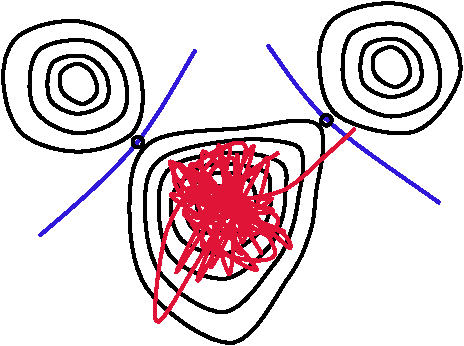
\includegraphics[width=0.9\textwidth]{images/rare-event}

    \end{column}

    \begin{column}[r]{0.5\textwidth}

      How to efficiency model the state-to-state dynamics? 

      \begin{itemize}
        \item Parallelize over time
        \item Accelerated Dynamics
          \begin{itemize}
            \item Alter potential energy surface
            \item Increase temperature
          \end{itemize}
        \item \alert<2>{Statistical mechanics}
      \end{itemize}
    \end{column}
  \end{columns}
  \vspace{2mm}
  \tiny
  Reproduced from Art Voter's ``Introduction to The Kinetic Monte Carlo Method''

\end{frame}


\begin{frame}{Kinetic Monte Carlo}

\begin{columns}[T]

\begin{column}{0.7\textwidth}
 Models state-to-state dynamics as a Markov chain
  \begin{itemize}
    \item The states must be Markovian
    \item Next event is chosen in proportion to its rate
    \item Escape time drawn from exponential distribution
      \[ P\left[\Delta t\right] = \exp \left( -\Delta t \sum_i \Gamma_i \right) \]
     \item Very fast (two random numbers and some book keeping)
  \end{itemize}
\end{column}

\begin{column}{0.3\textwidth}
	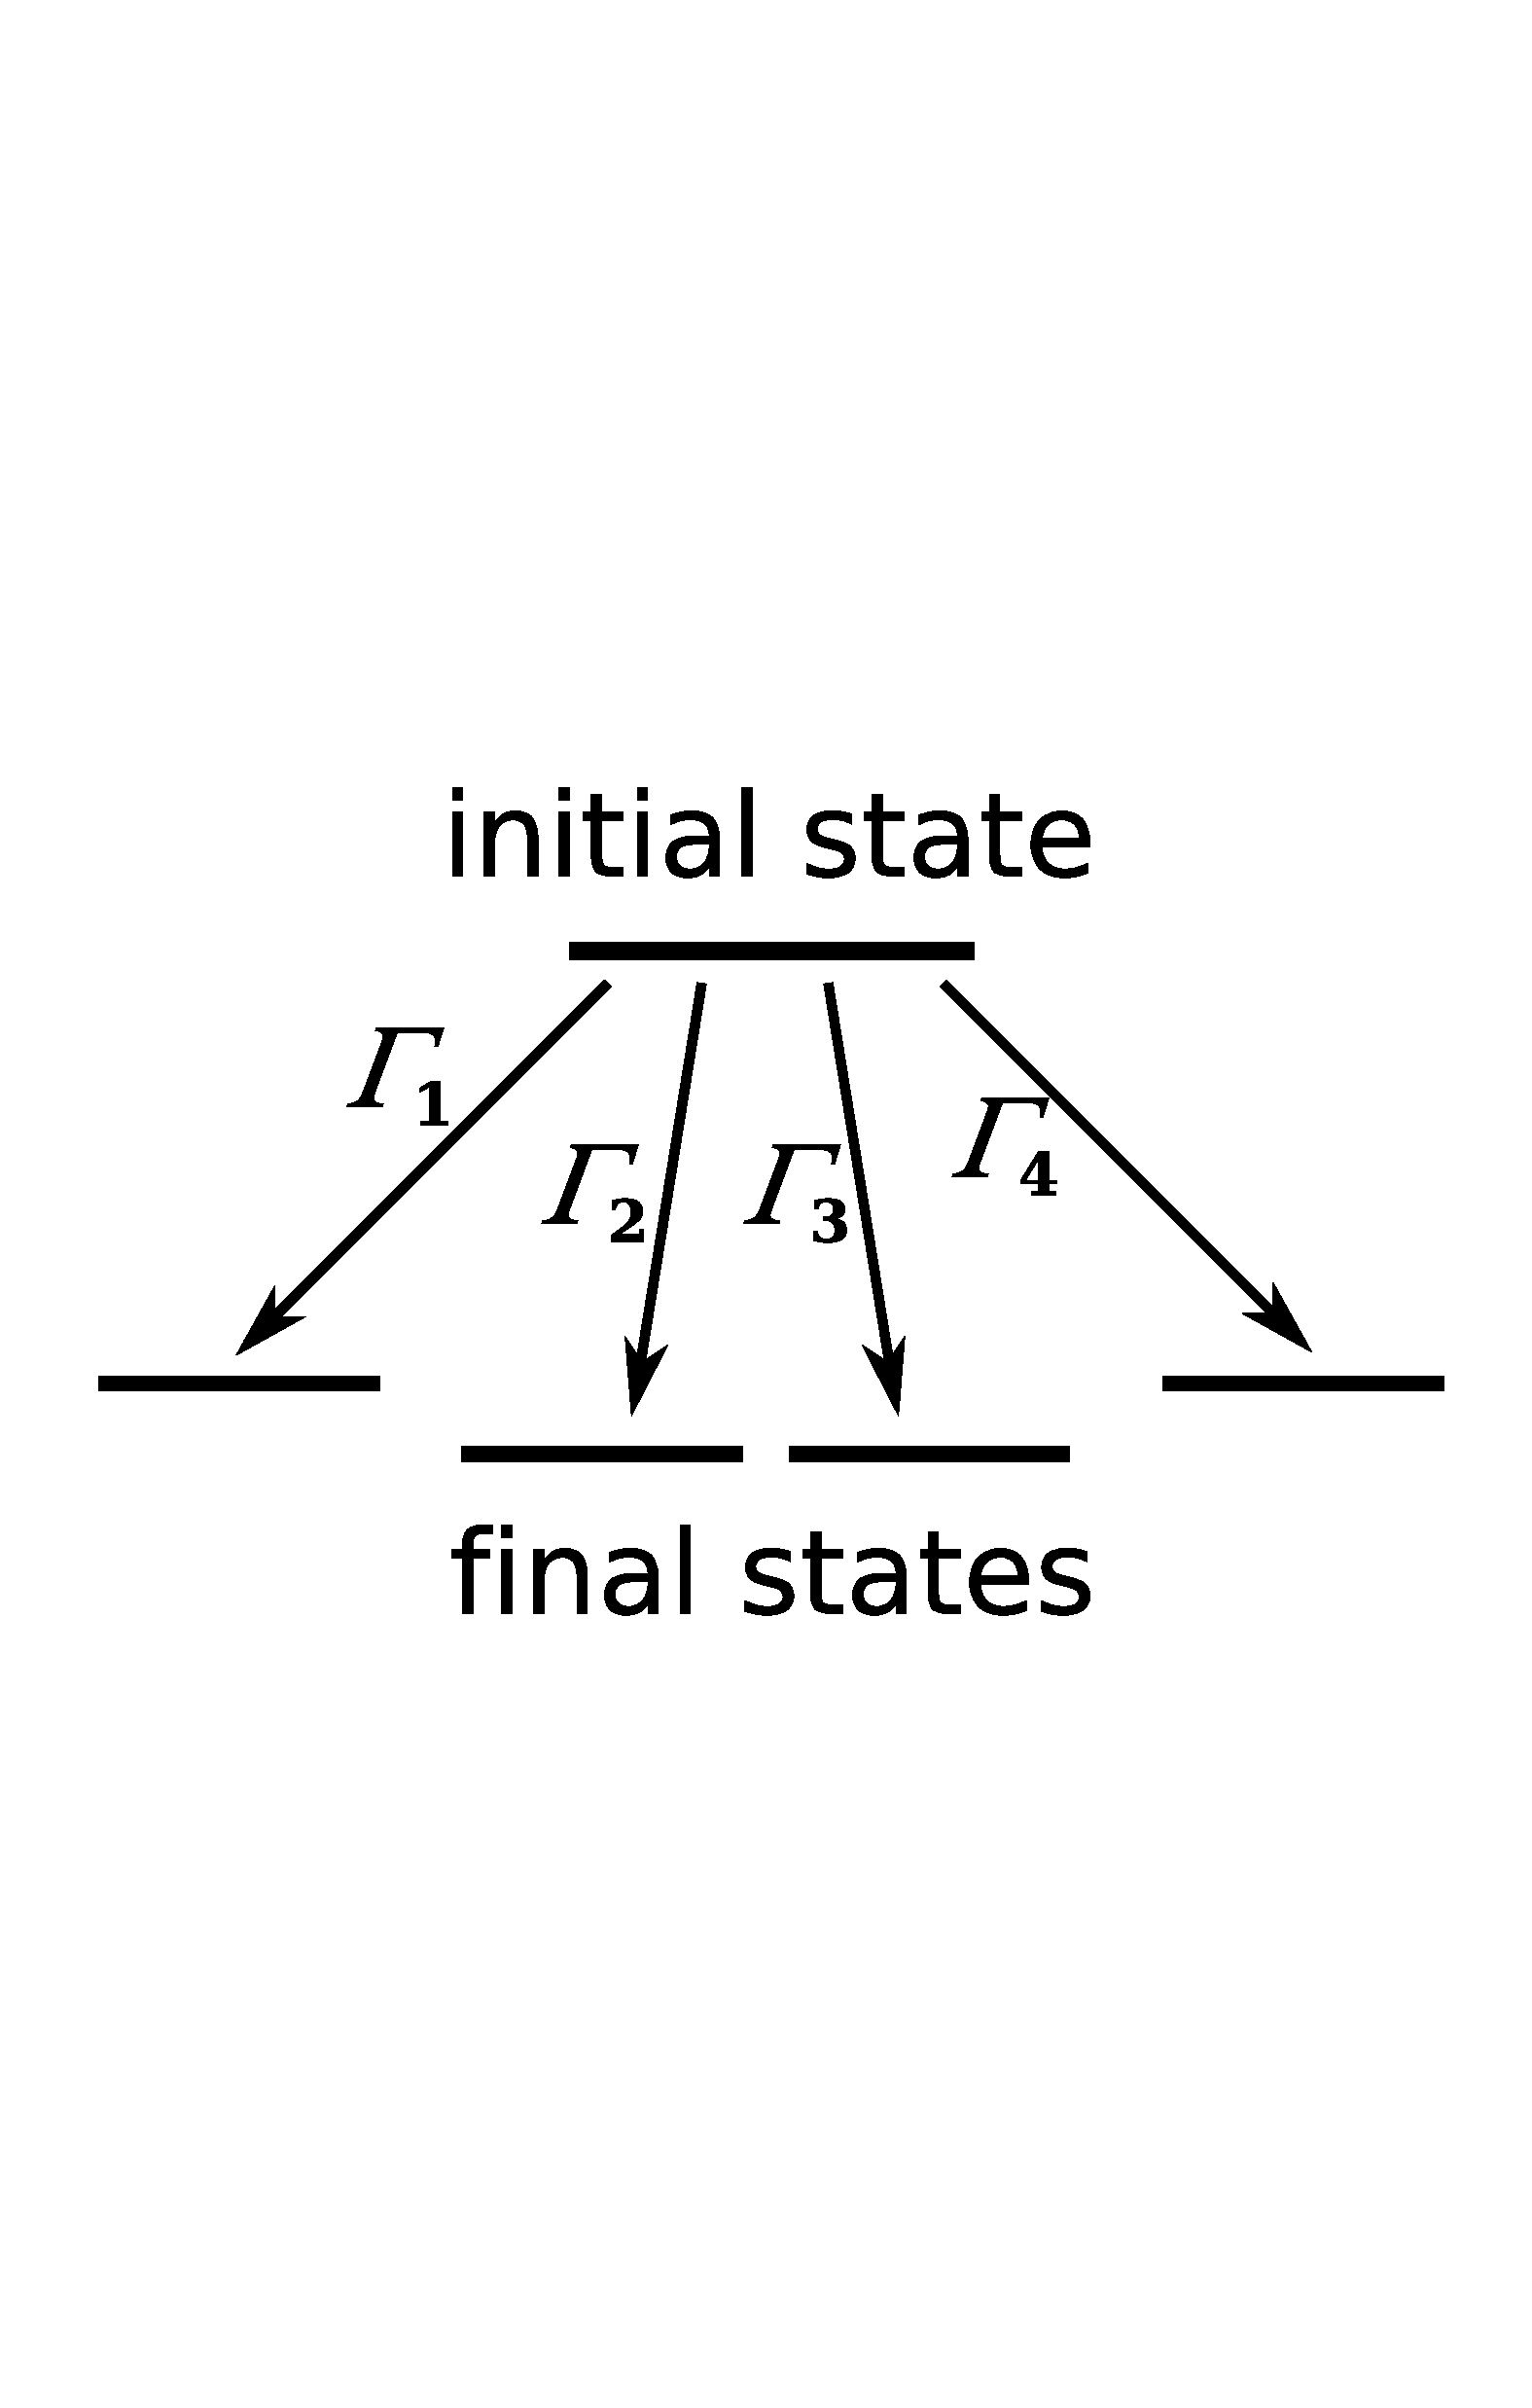
\includegraphics[width=\columnwidth]{images/kmc.pdf}
\end{column}

\end{columns}
\vspace{5mm}
How to build the Markov model? How to get the states and the rates?

\end{frame}


\begin{frame}{Adaptive Kinetic Monte Carlo}
 \begin{columns}
    \begin{column}[l]{0.65\textwidth}
\begin{tcolorbox}[title=Algorithm,colback=white,colframe=black,]
\begin{enumerate}
	\item \alert<2-3,11>{Displace randomly from the current minimum}
	\item \alert<4-5>{Min-mode saddle search (using dimer or Lanczos)}
	\item \alert<6>{Minimize along negative curvature at saddle to find new product state}
	\item \alert<7>{Ensure connectivity}
	\item \alert<8>{Calculate rate using HTST}
	\item \alert<9,11>{Estimate confidence that all important saddles have been found}
	\item \alert<10>{Take KMC steps until a new state is reached}
\end{enumerate}
\end{tcolorbox}
         \end{column}
    \begin{column}[r]{0.35\textwidth}
        \includegraphics<1>[width=\columnwidth]{images/pes.png}
        \includegraphics<2>[width=\columnwidth]{images/minmode-basins-2.pdf}
        \includegraphics<3>[width=\columnwidth]{images/minmode-basins-3.pdf}
        \includegraphics<4>[width=\columnwidth]{images/minmode-near-saddle.pdf}
        \includegraphics<5>[width=\columnwidth]{images/minmode-basins-4.pdf}
        \includegraphics<6>[width=\columnwidth]{images/minmode-basins-5.pdf}
        \includegraphics<7>[width=\columnwidth]{images/minmode-basins-6.pdf}
	 	        
        \only<8>{
        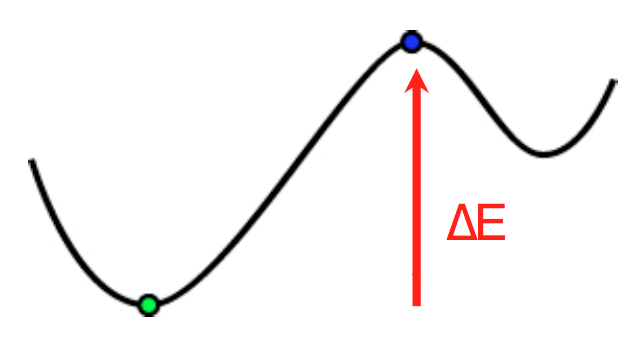
\includegraphics[width=\columnwidth]{images/barrier.png}
        
        \begin{equation*}
        r = A \exp \left[ -{\color{red}\Delta E}/k_\text{B} T \right]
	\end{equation*}
	}
	\only<9>{
		\begin{equation*}
		C = 1 - \frac{1}{N}
		\end{equation*}
		
		\vspace{2mm}
		
		$N$ is number of consecutive searches that did not find a new unique saddle 
	}
	\includegraphics<10>[width=\columnwidth]{images/kmc.pdf}
	
	\only<11>{Use high temperature MD to generate displacements.}


    \end{column}
  \end{columns}
\end{frame}

%\begin{frame}{Calculating Reaction Rates using HTST}
%
%  \begin{columns}
%    \begin{column}[l]{0.6\textwidth}
%      Use harmonic transition state theory (HTST) to calculate rates for solid state
%      systems:
%
%      \[
%        A = \frac{\prod_i^{3N} \nu_i^\text{min}}{\prod_i^{3N-1} \nu_i^\text{saddle}} 
%      \]
%
%      \[
%        r = \underbrace{A}_{\textrm{Attempt Freq.}} 
%        \underbrace{\exp \left[ -{\color{red}\Delta E}/k_\text{B} T \right]}_{\textrm{Boltzmann Probability}} 
%      \]
%    \end{column}
%
%    \begin{column}[r]{0.4\textwidth}
%      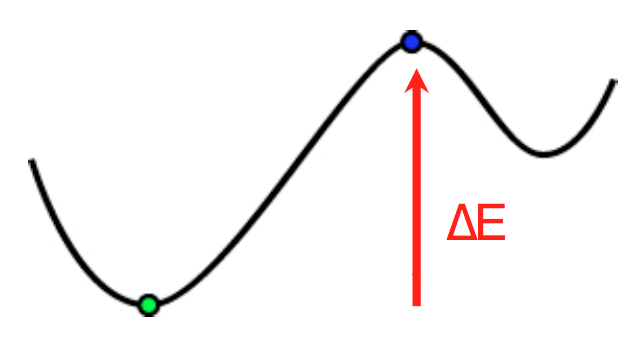
\includegraphics[width=1.0\textwidth]{images/barrier.png}
%    \end{column}
%  \end{columns}
%
%  \vspace{2mm}
%
%  Assumptions:
%  \begin{itemize}
%    \item Potential energy surface is harmonic
%    \item The reactant is in equilibrium with activated complex (saddle)
%    \item Trajectories at the saddle will always go to the product state (no recrossing)
%  \end{itemize}
%  
%  Works very well for solid state systems at low (room) temperature.
%
%\end{frame}



%\begin{frame}{Min-mode searches Pros and Cons}
% \begin{tcolorbox}[title=Pros,colback=white,colframe=green!50!black,]
%    \setbeamercolor{itemize item}{fg=black}
%    \begin{itemize}
%	\item Computationally cheap per search (3-4x minimization)
%	\item Easy to bias searches to subsets of atoms
%    \end{itemize}
%  \end{tcolorbox}
%
%  \vspace{2mm}
%
%  \begin{tcolorbox}[title=Cons,colback=white,colframe=red!50!black,]
%    \setbeamercolor{itemize item}{fg=black}
%    \begin{itemize}
%	\item Prior knowledge required to perform displacements
%	\item Can find saddles of high energy
%	\item Important events can be difficult to find
%	\item Difficult to estimate the error in the total rate
%	\item Easy to find saddles that are not connected to initial state
%    \end{itemize}
%  \end{tcolorbox}
%\end{frame}

\begin{frame}{Using High Temperature Molecular Dynamics to Find Saddles}


 \begin{columns}
    \begin{column}[l]{0.65\textwidth}
    Replace random displacements with MD displacements.
\begin{tcolorbox}[title=Algorithm,colback=white,colframe=black,]
\begin{enumerate}
	\item \alert<1>{Run high temperature MD}
	\item \alert<2>{Periodically minimize the system to see if it has exited}
	\item \alert<3-4>{Connect the initial minimum to the product minimum via a chain-of-states method such as Nudged Elastic Band}
	\item \alert<5>{Find first maxima along the minimized band}
\end{enumerate}
\end{tcolorbox}
	\end{column}
	\begin{column}{0.35\textwidth}
	
	\includegraphics<1>[width=\columnwidth]{images/md-escape-1.pdf}
	\includegraphics<2>[width=\columnwidth]{images/md-escape-2.pdf}
	\includegraphics<3>[width=\columnwidth]{images/md-escape-3.pdf}
	\includegraphics<4>[width=\columnwidth]{images/md-escape-4.pdf}
	\includegraphics<5>[width=\columnwidth]{images/md-escape-5.pdf}
	
	\end{column}
\end{columns}

\end{frame}


\begin{frame}{Estimating the Error in the Rate}

\begin{equation*}
C = \frac{R(t)}{R(\infty)} \approx 
 \frac{\left< R(t) \right>}{R(\infty)} \uncover<2->{ =
\frac{\displaystyle\sum_{i=1}^N r_i p_i(t)}{\displaystyle\sum_{i=1}^N r_i} \uncover<3>{\approx
\frac{\displaystyle\sum_{i \in F} r_i p_i(t)}{\displaystyle\sum_{i \in F} r_i}}}
\end{equation*}

$R(t)$: random variable of the total rate found after $t$ seconds
\uncover<2->{
\vspace{2mm}

$N$: total number of events

\vspace{2mm}

$p_i(t) = 1 - \exp(-tr^\mathrm{Hot}_i)$: probability that event $i$ has been found after $t$ seconds of high temperature MD

\vspace{2mm}

$r_i^\mathrm{Hot}$: can be calculated with HTST

\uncover<3->{
\vspace{2mm}

$F$: set of events that have been found
}
}

\end{frame}

\begin{frame}{Evaluating The Quality of the Error Estimator}

\begin{center}
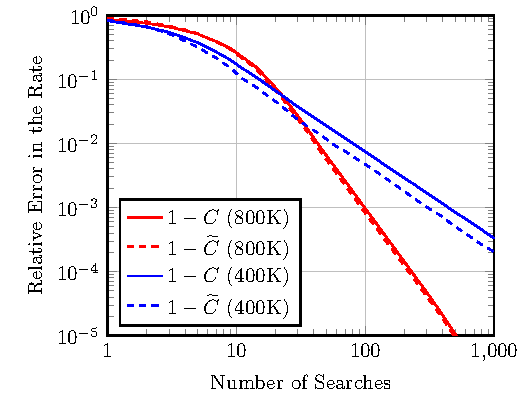
\includegraphics[width=0.55\textwidth]{images/confidence-test.pdf}
\end{center}

Times drawn from a harmonic system with rates calculated via HTST with 20 barriers linearly spaced between 0.1 and 0.4 eV.

Higher temperature sampling converges the total rate faster and reduces the bias of the estimator.

\end{frame}

\begin{frame}{Saddle Search Method Comparison}

\begin{columns}
\begin{column}{0.6\textwidth}
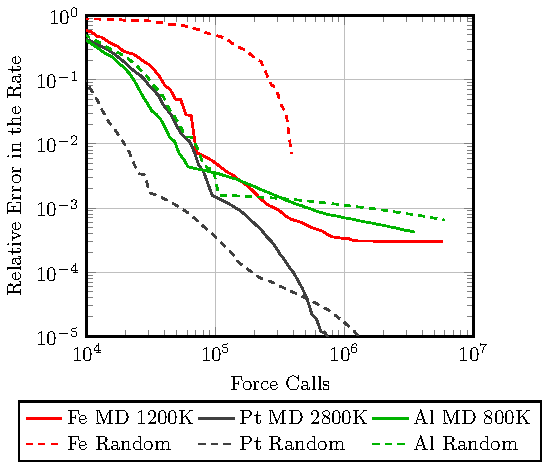
\includegraphics[width=\columnwidth]{images/saddle-search-comparison.pdf}
\end{column}
\begin{column}{0.4\textwidth}
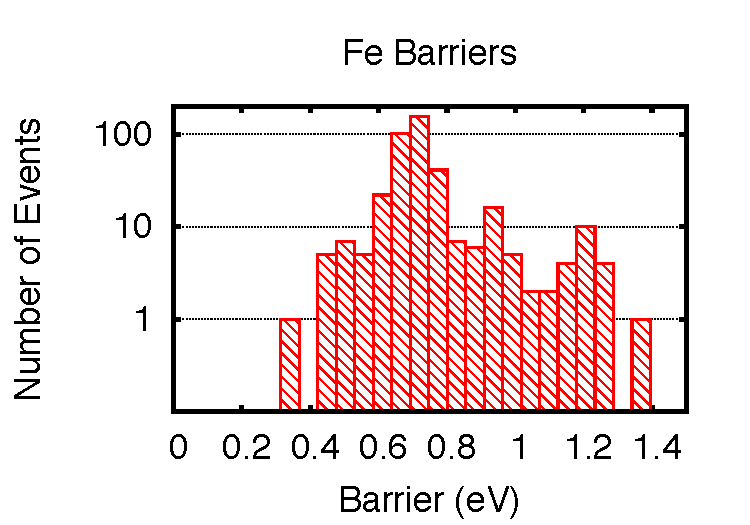
\includegraphics[width=\columnwidth]{images/fe-barriers.pdf}

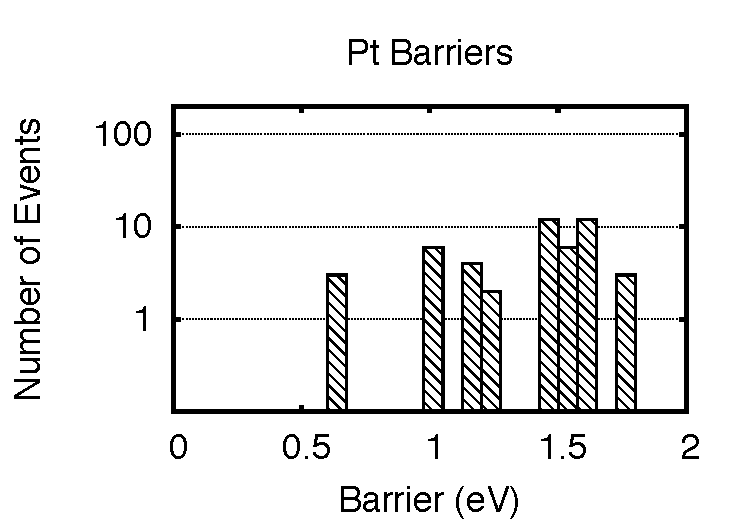
\includegraphics[width=\columnwidth]{images/pt-barriers.pdf}

\end{column}
\end{columns}

\end{frame}


\begin{frame}{Pros and Cons of MD Displacements compared to Random}
 \begin{tcolorbox}[title=Pros,colback=white,colframe=green!50!black,]
    \setbeamercolor{itemize item}{fg=black}
    \begin{itemize}
	\item Finds events with probability proportional to their rate
	\item Can estimate a confidence in the total rate found
	\item Reduced chance of finding disconnected events
	\item No prior knowledge needed about reaction coordinate
    \end{itemize}
  \end{tcolorbox}

  \vspace{2mm}

  \begin{tcolorbox}[title=Cons,colback=white,colframe=red!50!black,]
    \setbeamercolor{itemize item}{fg=black}
    \begin{itemize}
	\item MD displacement is more expensive than random
	\item NEB not guaranteed to find all pathways 
    \end{itemize}
  \end{tcolorbox}
\end{frame}

\begin{frame}{\textbf{Part II} A second class of rare event problems}
  \begin{block}{Superbasin}
    Superbasins are features of the potential energy surface, where there exist reactions that occur on widely differing timescales.
  \end{block}

  \begin{center}
    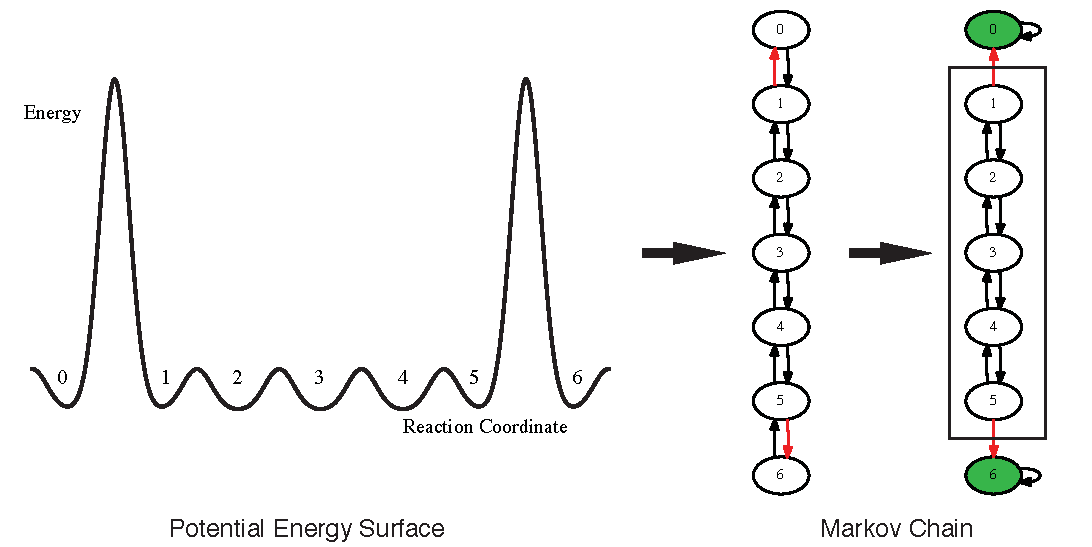
\includegraphics[width=0.95\textwidth]{images/superbasin-and-graphs}
  \end{center}

  %	  \begin{block}{Definition}
  %	
  %	    A superbasin is a collection of states with fast rates to the other states
  %	    in the superbasin and slow rates to exit the superbasin.
  %	
  %	  \end{block}

\end{frame}



\begin{frame}{Monte Carlo with Absorbing Markov Chains}

  The \emph{absorbing
  states}, $r$, are the exits from the superbasin and the \emph{transient
  states}, $s$, are within the superbasin. 
  \begin{equation*}
    \mathbf{M}_{(r+s) \times (r+s)} = 
    \left(
      \begin{array}{ c c }
        \mathbf{T}_{s\times s} & \mathbf{R}_{s\times r} \\
        \mathbf{0}_{r\times s} & \mathbf{I}_{r\times r} 
      \end{array}
    \right)
  \end{equation*}

  \vspace{3 mm}

  \begin{columns}[t]
    \begin{column}[l]{0.5\textwidth}
      Fundamental Matrix: mean number of times to visit state $j$ starting at state $i$
                  \vspace{-2mm}
      \begin{equation*}
        \mathbf{N}=\sum_{k=0}^\infty \mathbf{T}^k= {(\mathbf{I}-\mathbf{T})}^{-1} 
      \end{equation*}
      Mean time until absorption:
            \vspace{-2mm}
      \begin{equation*}
        \mathbf{t} = \mathbf{N} \mathbf{\tau} 
      \end{equation*}

      {$\tau$ is a vector of mean escape times from the transient states}
    \end{column}

    \begin{column}[r]{0.5\textwidth}
      Matrix of absorption probabilities:
      \begin{equation*}
        \mathbf{B}=\mathbf{N} \mathbf{R} 
      \end{equation*}
      $\mathbf{B}_{ij}$ is the probability of ending in state $j$ when starting in state $i$ 
    \end{column}
  \end{columns}

\end{frame}

\begin{frame}{Grouping States During a KMC Simulation}

  \begin{block}{Transition Counting}
    Identifying superbasins based on the number of times a transition has
    occurred.
  \end{block}

  \begin{center}
    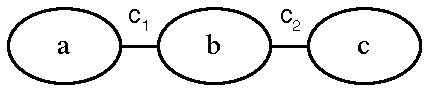
\includegraphics[width=0.5\textwidth]{images/tc.pdf}
  \end{center}

  Increment the counter $c_i$ each time a processes is followed. When
  $c_i \geq c_\mathrm{max}$ group the two states together.

  \begin{center}
    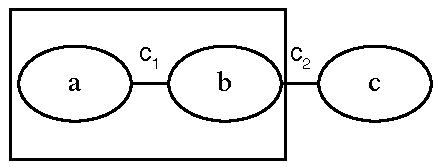
\includegraphics[width=0.5\textwidth]{images/tc2.pdf}
  \end{center}

\end{frame}

\begin{frame}{Modeling SiB$_2$ cluster break-up with AKMC and DFT}

States $a$ and $b$ form a superbasin that takes 5 billion steps to escape from on average at 300 K (about 20 days of computer time).

  \begin{center}
    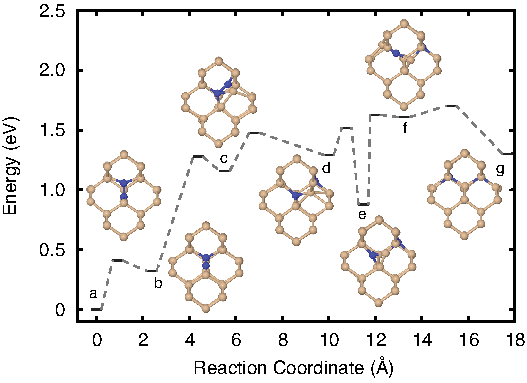
\includegraphics[width=0.7\textwidth]{images/sib2i-pes}
  \end{center}

\end{frame}

\begin{frame}{Performance of MCAMC}

When modeling events on disparate timescales, extended precision types are sometimes needed.

\begin{center}
\begin{tabular}{ r r r r r r}
\hline
N   & \texttt{float} (7) & \texttt{double} (16) & \texttt{dd} (32) & \texttt{qd} (64) & \texttt{arb.} (154) \\
\hline
10  & 0.0004 & 0.0002 & 0.0004  & 0.0016  & 0.0083 \\
100 & 0.0009 & 0.0011 & 0.0181  & 0.1768  & 1.0971 \\
200 & 0.0025 & 0.0038 & 0.0932  & 0.9876  & 5.8999 \\
500 & 0.0301 & 0.0439 & 1.1355  & 11.9715 & 64.7225 \\
800 & 0.0602 & 0.1065 & 3.6915  & 39.6592 & 247.9850 \\
\hline
\end{tabular}
\end{center}

Wall clock time in seconds for solving an absorbing Markov chain with N transient states. Computational effort is dominated by LU decomposition.

 \begin{tcolorbox}[title=Drunkard's Walk,colback=white,colframe=black,]
Open-source code for solving AMC problems in high precision.

\texttt{https://github.com/SamChill/drunkardswalk}
\end{tcolorbox}

\end{frame}


\begin{frame}{Eon: Open-source software for long timescale dynamics}

  Eon is software package that implements serveral long
  timescale dynamics methods. Details on obtaining the code at the end of this talk.

  \vspace{5 mm}

  \begin{columns}[T]
    \begin{column}[l]{0.5\textwidth}

      Methods
      \begin{itemize}
        \item Adaptive Kinetic Monte Carlo
        \item Parallel Replica
        \item Hyper Dynamics (Bond Boost)
        \item Basin Hopping
        \item $\kappa$-dynamics (in progress)
        \item Temperature Accelerated Dynamics (in progress)
      \end{itemize}
    \end{column}
    \begin{column}[r]{0.5\textwidth}
      Parallelization Options
      \begin{itemize}
        \item Local
        \item Job Queuing System (PBS, SGE, etc)
        \item BOINC (Distributed Computing)
        \item MPI
      \end{itemize}

    \end{column}
  \end{columns}

  \vspace{5 mm}

  Potentials: EAM, LAMMPS, GPAW, VASP, and others.

\end{frame}
%
%
%
%
%\begin{frame}{Parallel AKMC}
%    \includegraphics[width=\textwidth]{figures/parallel-akmc.png}
%
%    Each job is an independent calculation. Additionally, the evaluation of
%    the forces can be parallelized for each job. For systems of
%    practical interest up to a thousands jobs can be run in parallel with
%    perfectly linear scaling.
%
%\end{frame}
%
%\begin{frame}{BOINC Project}
%\begin{center}
%\includegraphics[width=0.35\textwidth]{figures/boinc.png}
%\end{center}
%
%We have a distributed computing project: http://eon.ices.utexas.edu
%
%\begin{itemize}
%\item $\sim1400$ computers 
%\item $\sim4500$ cores total
%\item $\sim4.5$ Teraflops
%\item Don't have to pay \$\$\$
%\end{itemize}
%
%We have a medium sized computer lab on campus attached to our project as well
%as idle computer time from a computing facility at the University of Houston.
%
%\end{frame}
%
%
%\begin{frame}{Running on Massively Parallel Computers}
%\begin{columns}
%\begin{column}[l]{0.4\textwidth}
%    \includegraphics[width=0.9\textwidth]{figures/intrepid.jpg}
%\end{column}
%\begin{column}[r]{0.6\textwidth}
%    \begin{itemize}
%        \item Enables the use of DFT instead of empirical FF
%        \item How to run the server, client, and potentials as one job?
%        \begin{itemize}
%            \item Use Multiple Program Multiple Data (MPMD) MPI
%            \item The server, client, and potential ranks run as one MPI job
%            \item Must modify the potential code to get it to play along
%            \item Currently have VASP and GPAW working
%        \end{itemize}
%    \end{itemize}
%
%\end{column}
%\end{columns}
%
%\begin{center}
%    \begin{eqnarray*}
%    {\color{red}\left[100;1,000\right]\textsc{jobs}} &*& {\color{blue}\left[8;512\right] \frac{\textsc{cores}}{\textsc{job}}} = \left[800;512,000\right] \textsc{cores} \\
%    {\color{red}\textsc{AKMC}}&& {\color{blue}\textsc{DFT}}
%    \end{eqnarray*}
%\end{center}
%
%Intrepid has 163,840 cores and Mira will have 768,000 cores.
%\end{frame}
%
%\begin{frame}{DFT AKMC Performance}
%
%\includegraphics[width=0.9\textwidth]{figures/dft-akmc-scaling.pdf}
%
%\end{frame}
%
%
%\begin{frame}{Conclusion}
%\begin{itemize}
%    \item MCAMC treats superbasins exactly
%    \item Can use a simple scheme to classify superbasins on the fly
%    \item Eon is an opensource software package for long timescale dynamics
%    \begin{itemize}
%    	  \item Adaptive kinetic Monte Carlo
%	  \item Parallel Replica
%	  \item Hyperdynamics (Bond Boost)
%	  \item Basin hopping (global optimization)
%	\end{itemize}
%	  
%\end{itemize}
%
%\end{frame}
%
%

\begin{frame}{Eon Homepage: \texttt{http://theory.cm.utexas.edu/eon}}
  \begin{center}
    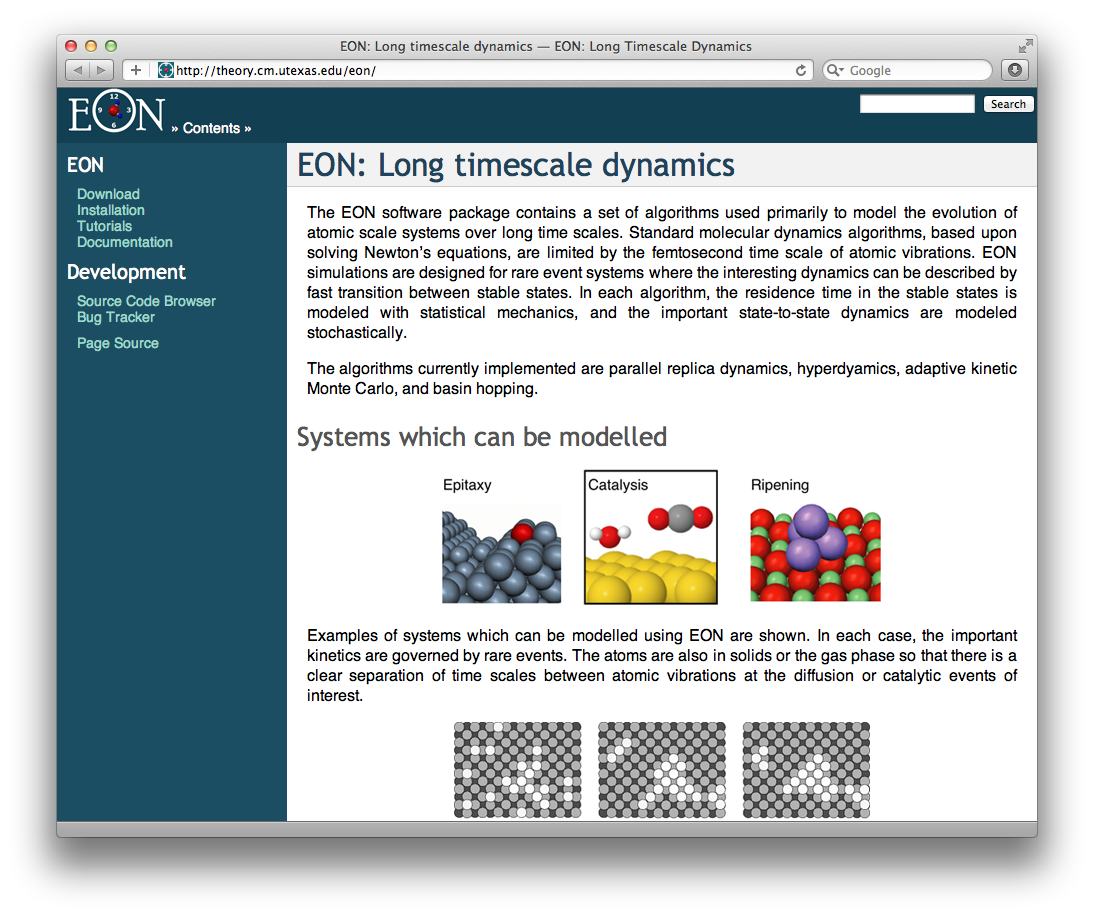
\includegraphics[width=0.6\textwidth]{images/eon-website.png}
  \end{center}
  \small{S. T. Chill,  M. Welborn, R. Terrell, L. Zhang, J. C. Berthet, A. Pedersen, H. Jonsson, and G. Henkelman \textit{Model. Simul. Mater. Sci. Eng}, \textbf{Submitted 2013}.}
\end{frame}

%
%
%\begin{frame}{Parallel Replica Dynamics}
%
%
%  \begin{tcolorbox}[title=Pros,colback=white,colframe=green!50!black,]
%    \setbeamercolor{itemize item}{fg=black}
%    \begin{itemize}
%      \item Can be as accurate as vanilla MD
%      \item Simple to implement
%      \item Scales well with number of CPUs
%      \item Can be used with other accelerated MD methods (hyperdynamics)
%    \end{itemize}
%  \end{tcolorbox}
%
%  \vspace{2mm}
%
%  \begin{tcolorbox}[title=Cons,colback=white,colframe=red!50!black,]
%    \setbeamercolor{itemize item}{fg=black}
%    \begin{itemize}
%      \item No acceleration per CPU
%      \item How to efficiently draw replicas from QSD
%      \item Does not address hierarchy of rare event problems
%    \end{itemize}
%  \end{tcolorbox}
%
%\end{frame}
%
%\begin{frame}{Hyperdynamics}
%
%  \begin{tcolorbox}[title=Pros,colback=white,colframe=green!50!black,]
%    \setbeamercolor{itemize item}{fg=black}
%    \begin{itemize}
%      \item Can be as accurate as vanilla MD (tricky, see below) 
%      \item Exponential speedup to see escapes (depends on bias potential)
%    \end{itemize}
%  \end{tcolorbox}
%
%  \vspace{2mm}
%
%  \begin{tcolorbox}[title=Cons,colback=white,colframe=red!50!black,]
%    \setbeamercolor{itemize item}{fg=black}
%    \begin{itemize}
%      \item Does not address hierarchy of rare event problems
%    \end{itemize}
%    How to construct good bias potential?
%    \begin{itemize}
%      \item Must go to zero at transition surface
%      \item Exponential average must converge
%      \item Boost should still be large
%    \end{itemize}
%  \end{tcolorbox}
%
%\end{frame}
%
%\begin{frame}{Temperature Accelerated Dynamics}
%  \begin{tcolorbox}[title=Pros,colback=white,colframe=green!50!black,]
%    \setbeamercolor{itemize item}{fg=black}
%    \begin{itemize}
%      \item Exponential speedup
%      \item Requires less prior knowledge than hyperdynamics
%    \end{itemize}
%  \end{tcolorbox}
%
%  \vspace{2mm}
%
%  \begin{tcolorbox}[title=Cons,colback=white,colframe=red!50!black,]
%    \setbeamercolor{itemize item}{fg=black}
%    \begin{itemize}
%      \item hTST must hold at the dynamics temperature (typically large)
%      \item Does not address hierarchy of rare event problems
%    \end{itemize}
%  \end{tcolorbox}
%\end{frame}
%
%\begin{frame}{Adaptive Kinetic Monte Carlo}
%  \begin{tcolorbox}[title=Pros,colback=white,colframe=green!50!black,]
%    \setbeamercolor{itemize item}{fg=black}
%    \begin{itemize}
%      \item Large speedups compared to molecular dynamics
%      \item Calculate temperature dependence with minimal effort
%      \item Re-use information from previous states (recycling, KDB)
%      \item Quickly calculate time distributions from Markov chain
%    \end{itemize}
%  \end{tcolorbox}
%
%  \vspace{1mm}
%
%  \begin{tcolorbox}[title=Cons,colback=white,colframe=red!50!black,]
%    \setbeamercolor{itemize item}{fg=black}
%    \begin{itemize}
%      \item hTST must hold at the simulation temperature
%      \item How to ensure states are Markovian?
%      \item \Ovalbox{Difficulty in calculating confidence/error}
%      \item \Ovalbox{How to find the important events without prior knowledge}
%      \item \Ovalbox{Does not address hierarchy of rare event problems}
%    \end{itemize}
%  \end{tcolorbox}
%\end{frame}
%
%\begin{frame}{Method Comparison}
%
%
%  \begin{center}
%    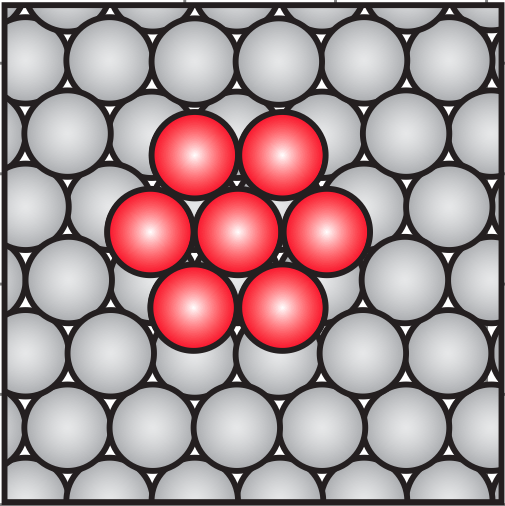
\includegraphics[width=32mm]{images/pt-island.png}
%  \end{center}
%
%  \begin{center}
%    \begin{tabular*}{0.8\columnwidth}{l @{\extracolsep{\fill}} c c}
%      \hline
%      Method & Escape Rate (1/s) & Force Calls \\
%      \hline
%      Parallel Replica & (7.7 $\pm$ 3.8)$\e{5}$ &  1$\e{9}$ \\
%      Parallel Replica / HD & (3.4 $\pm$ 1.7)$\e{5}$ & 1$\e{7}$ \\
%      AKMC & 7.0$\e{5}$ & 2$\e{4}$ \\
%      \hline
%    \end{tabular*}
%  \end{center}
%
%
%  Comparison of the rate of escape from
%  the Pt heptamer island state at 400K using different long timescale methods.
%
%\end{frame}


\end{document}


